\documentclass[12pt]{article}%
\usepackage{amsfonts}
\usepackage{fancyhdr}
\usepackage[a4paper, top=2.5cm, bottom=2.5cm, left=2.2cm, right=2.2cm]%
{geometry}
\usepackage{amsmath}
\usepackage{amssymb}
\usepackage{caption,subcaption}
\usepackage{graphicx}%
\newcommand{\indicator}{\mathbb{I}} 
\newcommand{\expectation}{\mathbb{E}} 
\newcommand{\bs}{\boldsymbol}

\DeclareMathOperator*{\argmax}{arg\,max}
\DeclareMathOperator*{\argmin}{arg\,min}

\begin{document}

\title{Assignment 2: HMM for Categorical Data Sequences}
\author{Miguel Fern\'{a}ndez D\'{i}az}
\date{\today}
\maketitle
\section{Expression for the complete data log-likehood for the N sequences}
According to this expression for the complete data log-likelihood
\begin{equation}
\label{ll1}
l_{c}\left(\boldsymbol\theta\right) = \log p ( S , Y | \boldsymbol\theta ) = \log \prod _ { n = 1 } ^ { N } \left( p \left( s _ { 1 } ^ { n } | \boldsymbol\pi \right) \prod _ { t = 2 } ^ { T _ { n } } p \left( s _ { t } ^ { n } | s _ { t - 1 } ^ { n } , \mathbf { A } \right) \right) \left( \prod _ { t = 1 } ^ { T _ { n } } p \left( \mathbf { y } _ { t } ^ { n } | s _ { t } ^ { n } , \mathbf { B } \right) \right)
\end{equation}
where log operator is the Naperian logarithm, $S$ represents the hidden states of the model, $Y$ is the observed continuous sequence, $\mathbf { A }$ stands for the state transition probabilities,$B$ the observatoin emission probabilites and $\boldsymbol\pi$ is the initial state probability distribution. \\

\noindent The parameters of the model are
\begin{equation}
\boldsymbol\theta = \{ \mathbf { A } , \mathbf { B } , \boldsymbol\pi \}.
\end{equation}
Equation \eqref{ll1} is composed by three main terms: the $\boldsymbol\pi$, $\mathbf { A }$ and $\mathbf { B } $ ones which can be rewritten as
\begin{align}
p \left( s _ { 1 } ^ { n } | \boldsymbol\pi \right) &= \prod\limits_{k=1}^{K}\pi_{k}^{\indicator \lbrace s_{1}^{n}=k|Y,\boldsymbol\theta\rbrace},\\
p \left( s _ { t } ^ { n } | s _ { t - 1 } ^ { n } , \mathbf { A } \right) &= \prod\limits_{k=1}^{K} \prod\limits_{k'=1}^{K}a_{k,k'}^{\indicator \lbrace s_{t-1}^{n}=k,s_{t}^{n}=k'|Y,\boldsymbol\theta\rbrace},\\
p \left( \mathbf { y } _ { t } ^ { n } | s _ { t } ^ { n } , \mathbf { B } \right) &= \prod\limits_{k=1}^{K} p \left( \mathbf { y } _ { t } ^ { n } | \boldsymbol b_{k} \right) = \prod\limits_{k=1}^{K} p \left( \mathbf { y } _ { t } ^ { n } | \boldsymbol\theta_{k} \right) \label{p3LL}.
\end{align}
In this case, $\indicator$ represents an indicator function, $k = \lbrace{1,...,K}\rbrace$ the current latent state of the model, $a_{k,k'}$ the $k$th row and $k'$th column element of the forementioned matrix $\mathbf { A }$, $t = \lbrace{1,...,T_{n}}\rbrace$ the position of the state in sequence $n$. Please notice that now, $\mathbf{b}_{k}$ (that belonged to $\mathbf{B}$ becomes $\boldsymbol\theta_{k}$, which denotes the hyperparameters of the categorical distribution that the data follow.\\

\noindent Since our data follow a categorical distribution, equation (\ref{p3LL}) can be expressed as
\begin{equation}
p \left( \mathbf { y } _ { t } ^ { n } | \boldsymbol\theta_{k} \right) = \prod\limits_{j=1}^{Dt} \text{Cat}(y_{j,t}|\boldsymbol\theta_{k}).
\end{equation}
With a further development we can get
\begin{equation}
p \left( \mathbf { y } _ { t } ^ { n } | \boldsymbol\theta_{k} \right) = \prod\limits_{j=1}^{Dt} \text{Cat}(y_{j,t}|\boldsymbol\theta_{k}) = \prod\limits_{m=1}^{I}\prod\limits_{j=1}^{Dt}\theta_{k,m}^{\indicator\lbrace{y_{j,t}^{n}=m}\rbrace} = \prod\limits_{m=1}^{I}\theta_{k,m}^{\sum\limits_{j=1}^{Dt}\indicator\lbrace{y_{j,t}^{n}=m}\rbrace} = \prod\limits_{m=1}^{I}\theta_{k,m}^{\mu^{n}_{t,m}},
\end{equation}
being $\mu^{n}_{t,m}$
\begin{equation}
\mu^{n}_{t,m} = \sum\limits_{j=1}^{Dt}\indicator\lbrace{y_{j,t}^{n}=m}\rbrace.
\end{equation}
So the complete data log-likelihood is written in this way
\begin{equation}
\begin{split}
l_{c}\left(\boldsymbol\theta\right) &= \sum\limits_{n=1}^{N}\sum\limits_{k=1}^{K}\indicator \lbrace s_{1}^{n}=k|Y,\boldsymbol\theta\rbrace \log(\pi_{k}) + \\
&+ \sum\limits_{n=1}^{N}\sum\limits_{k=1}^{K}\sum\limits_{k'=1}^{K}\sum\limits_{t=1}^{T_{n}}\indicator \lbrace s_{t-1}^{n}=k,s_{t}^{n}=k'|Y,\boldsymbol\theta\rbrace \log(a_{k,k'}) + \\
&+ \sum\limits_{n=1}^{N}\sum\limits_{t=1}^{T_{n}}\indicator \lbrace s_{t}^{n}=k|Y,\boldsymbol\theta\rbrace \sum\limits_{m=1}^{I}\mu^{n}_{t,m} \log(\theta_{k,m}).
\end{split}
\end{equation}
\section{Expression for the expected complete data log likelihood}
The expected complete data log-likelihood has the following form
\begin{equation}
Q \left( \boldsymbol { \theta } , \boldsymbol { \theta } ^ { t - 1 } \right) = E \left\{ l _ { c } ( \boldsymbol { \theta } ) | \mathcal { D } , \boldsymbol { \theta } ^ { t - 1 } \right\}
\end{equation}
As in the previous section, and considering the nature of $l_{c}$ and its three main components, this expectation calculation can be divided in three.
\begin{align}
& \expectation \left( \sum _ { n = 1 } ^ { N } \indicator \left( s _ { 1 } ^ { n } = k | Y , \bs\theta \right) \right) = \sum _ { n = 1 } ^ { N } \gamma _ { n , 1 } ( k ), \\
& \expectation \left( \sum _ { n = 1 } ^ { N } \sum _ { t = 2 } ^ { T _ { n } } \indicator \left( s _ { t - 1 } ^ { n } = k , s _ { t } ^ { n } = k' | Y , \bs\theta \right) \right) = \sum _ { n = 1 } ^ { N } \sum _ { t = 2 } ^ { T _ { n } } \xi _ { n , t } ( k , k' ), \\
& \expectation \left( \sum _ { n = 1 } ^ { N } \sum _ { t = 1 } ^ { T _ { n } } \indicator \left( s _ { t } ^ { n } = k | Y , \bs\theta \right) \right) = \sum _ { n = 1 } ^ { N } \sum _ { t = 1 } ^ { T _ { n } } \gamma _ { n , t } ( k ).
\end{align}
Where 
\begin{equation}
\sum _ { k = 1 } ^ { K } \gamma _ { n , t } ( k ) = 1.
\end{equation}
\noindent Being $\xi _ { n,t } ( k , k' )$ 
\begin{equation}
\xi _ { n,t } ( k , k' ) = \alpha _ { t-1 }^{n} ( k ) a _ { k,k' } \prod\limits_{m=1}^{I} \theta_{k,m}^{\mu^{n}_{t,m}} \beta _ { t }^{n} ( k' ),
\end{equation}
and $ \gamma _ { n , t } ( k ) $
\begin{equation}
\gamma _ { n , t } ( k )\propto \beta _ { t }^{n} ( k )\alpha _ { t }^{n} ( k )
\end{equation}
The terms $\alpha$ and $\beta$ are computed by means of the forward-backward algorithm as follows
\begin{align}
\label{alfabeta}
&\alpha _ { 1 }^{n} ( k ) = \pi _ { k } \prod\limits_{m=1}^{I}\theta_{k,m}^{\mu^{n}_{1,m}}, \\
&\alpha _ { t }^{n} ( k ) = \left( \sum _ { k' = 1 } ^ { K } \alpha _ { t - 1 }^{n} ( k' ) a _ { k',k } \right) \prod\limits_{m=1}^{I}\theta_{k,m}^{\mu^{n}_{t,m}}, \\
&\beta _ { T_{n} }^{n} ( k ) = 1, \\
& \beta _ { t }^{n} ( k ) = \sum _ {k' = 1 } ^ { K } a _ { k,k'}  \prod\limits_{m=1}^{I}\theta_{k',m}^{\mu^{n}_{t+1,m}}  \beta _ { t + 1 }^{n} ( k' ).
\end{align}
So the complete expression for $Q \left( \boldsymbol { \theta } , \boldsymbol { \theta } ^ { t - 1 } \right)$ is now
\begin{equation}
\begin{split}
Q \left( \boldsymbol { \theta } , \boldsymbol { \theta } ^ { t - 1 } \right) &= \sum\limits_{k=1}^{K}\sum _ { n = 1 } ^ { N } \gamma _ { n , 1 } ( k ) \log(\pi_{k}) + \\
&+ \sum\limits_{k=1}^{K}\sum\limits_{k'=1}^{K}\sum _ { n = 1 } ^ { N } \sum _ { t = 2 } ^ { T _ { n } } \xi _ { n , t } ( k , k' ) \log(a_{k,k'}) + \\
&+ \sum\limits_{k=1}^{K}\sum\limits_{m=1}^{I}\sum _ { n = 1 } ^ { N } \sum _ { t = 1 } ^ { T _ { n } } \gamma _ { n , t } ( k )\mu^{n}_{t,m} \log(\theta_{k,m}).
\end{split}
\end{equation}
\section{Maximum Likelihood estimation of the parameters of the model}
There are three parameters for the model, which are $\mathbf{A}$, $\bs\theta$ and $\bs\pi$, and they are computed by means of Lagrange multipliers.
\subsection{ML estimation of $\pi_{k}$}
In order to compute $\pi_{k}$, we first need to take into account the following restrictions
\begin{align}
& 0 \leq \pi_{k} \leq 1 \\
& \sum\limits_{k = 1}^{K} \pi_{k} = 1.
\end{align}
Now, let us define the lagrangian as
\begin{equation}
\label{lagrange_pik}
L\left( Q(\pi_{k}),\lambda \right) = Q(\pi_{k}) + \lambda \left( \sum \limits_{k=1}^{K} \pi_{k} - 1 \right),
\end{equation}
which will be optimized in this way
\begin{equation}
\label{minmax_lagrange_pik}
\min_{\substack{\lambda}} \max_{\substack{\pi_{k}}} \lbrace L\left( Q(\pi_{k}),\lambda \right) \rbrace.
\end{equation}
By first taking the derivative with respect to $\pi_{k}$ and equating it to 0
\begin{equation}
\label{deriv_pik}
\begin{split}
& \dfrac{\partial L}{\partial \pi_{k}} = 0 = \sum \limits_{n=1}^{N} \dfrac{\gamma_{n,1}(k)}{\pi_{k}} - \lambda, \\
& \pi_{k} = \dfrac{1}{\lambda} \sum \limits_{n=1}^{N} \gamma_{n,1}(k).
\end{split}
\end{equation}
And later with respect to $\lambda$
\begin{equation}
\begin{split}
& \dfrac{\partial L}{\partial \lambda} = 0 = \sum \limits_{k=1}^{K} \pi_{k} - 1,\\
& \sum \limits_{k=1}^{K} \pi_{k} = 1.\\
\end{split}
\end{equation}
Taking into account the previous equation, if in both sides of \eqref{deriv_pik} summatories all over $K$ are taken, then the value of $\lambda$ can be obtained
\begin{equation}
\begin{split}
& \sum \limits_{k=1}^{K}\pi_{k} = \sum \limits_{k=1}^{K} \dfrac{1}{\lambda} \sum \limits_{n=1}^{N} \gamma_{n,1}(k)\\
& 1 = \dfrac{1}{\lambda} \sum \limits_{n=1}^{N}\sum \limits_{k=1}^{K}\gamma_{n,1}(k).\\
\end{split}
\end{equation}
Now, considering the previously imposed restrictions and recalling that
\begin{equation}
\sum _ { k = 1 } ^ { K } \gamma _ { n , t } ( k ) = 1,
\end{equation}
the value of $\lambda$ is
\begin{equation}
\begin{split}
& 1 = \dfrac{1}{\lambda} \sum \limits_{n=1}^{N}1.\\
& \lambda = N.\\
\end{split}
\end{equation}
And with that value of $\lambda$ the estimated value of $\pi_{k}$ is
\begin{equation}
\widehat{\pi}_{k} = \dfrac{1}{N} \sum \limits_{n=1}^{N} \gamma_{n,1}(k).
\end{equation}
\subsection{ML estimation of $\theta_{k,m}$}
Now, the parameter to be estimated is $\theta_{k,m}$ and the constraint is now
\begin{equation}
\label{constraint_thetakm}
\sum \limits_{m=1}^{I} \theta_{k,m} = 1.
\end{equation}
Being the whole expression
\begin{equation}
\label{lagrange_thetakm}
L\left( Q(\theta_{k,m}),\lambda \right) = Q(\theta_{k,m}) + \lambda \left( \sum \limits_{m=1}^{I} \theta_{k,m} - 1 \right),
\end{equation}
which will be optimized in this way
\begin{equation}
\label{minmax_lagrange_thetakm}
\min_{\substack{\lambda}} \max_{\substack{\theta_{k,m}}} \lbrace L\left( Q(\theta_{k,m}),\lambda \right) \rbrace.
\end{equation}
By first taking the derivative with respect to $\theta_{k,m}$ and equating it to 0
\begin{equation}
\label{deriv_thetakm}
\begin{split}
& \dfrac{\partial L}{\partial \theta_{k,m}} = 0 = \sum \limits_{n=1}^{N}\sum _ { t = 1 } ^ { T _ { n } } \dfrac{\gamma_{n,t}(k)\mu_{t,m}^{n}}{\theta_{k,m}} - \lambda, \\
& \theta_{k,m} = \dfrac{1}{\lambda} \sum \limits_{n=1}^{N} \sum _ { t = 1 } ^ { T _ { n } }\gamma_{n,t}(k)\mu_{t,m}^{n}.
\end{split}
\end{equation}
And later with respect to $\lambda$
\begin{equation}
\begin{split}
& \dfrac{\partial L}{\partial \lambda} = 0 = \sum \limits_{m=1}^{I} \theta_{k,m} - 1,\\
& \sum \limits_{m=1}^{I} \theta_{k,m} = 1.\\
\end{split}
\end{equation}
Taking into account the previous equation, if in both sides of \eqref{deriv_thetakm} summatories all over $I$ are taken, then the value of $\lambda$ can be obtained
\begin{equation}
\begin{split}
& \sum \limits_{m=1}^{I}\theta_{k,m} = \sum \limits_{m=1}^{I} \dfrac{1}{\lambda} \sum \limits_{n=1}^{N}\sum _ { t = 1 } ^ { T _ { n } } \gamma_{n,t}(k)\mu_{t,m}^{n}\\
& 1 = \dfrac{1}{\lambda} \sum \limits_{n=1}^{N}\sum _ { t = 1 } ^ { T _ { n } }\sum \limits_{m=1}^{I}\gamma_{n,t}(k)\mu_{t,m}^{n},\\
& \lambda = \sum \limits_{n=1}^{N}\sum \limits_{ t = 1 } ^ { T _ { n }}\sum \limits_{m=1}^{I}\gamma_{n,t}(k)\mu_{t,m}^{n}.\\
\end{split}
\end{equation}
And with that value of $\lambda$ the estimated value of $\theta_{k,m}$ is
\begin{equation}
\widehat{\theta}_{k,m} = \dfrac{\sum \limits_{n=1}^{N} \sum \limits_ { t = 1 } ^ { T _ { n } }\gamma_{n,t}(k)\mu_{t,m}^{n}}{\sum \limits_{n=1}^{N}\sum \limits_ { t = 1 } ^ { T _ { n } }\sum \limits_{m=1}^{I}\gamma_{n,t}(k)\mu_{t,m}^{n}}.
\end{equation}
\subsection{ML estimation of $a_{k,k'}$}
At last, the parameter to be estimated is $a_{k,k'}$ and the constraint is now
\begin{equation}
\label{constraint_akk}
\sum \limits_{k'=1}^{K} a_{k,k'} = 1.
\end{equation}
Being the whole expression
\begin{equation}
\label{lagrange_akk}
L\left( Q(a_{k,k'}),\lambda \right) = Q(a_{k,k'}) + \lambda \left( \sum \limits_{k'=1}^{K} a_{k,k'} - 1 \right),
\end{equation}
which will be optimized in this way
\begin{equation}
\label{minmax_lagrange_akk}
\min_{\substack{\lambda}} \max_{\substack{a_{k,k'}}} \lbrace L\left( Q(a_{k,k'}),\lambda \right) \rbrace.
\end{equation}
By first taking the derivative with respect to $a_{k,k'}$ and equating it to 0
\begin{equation}
\label{deriv_akk}
\begin{split}
& \dfrac{\partial L}{\partial a_{k,k'}} = 0 = \sum \limits_{n=1}^{N}\sum _ { t = 2 } ^ { T _ { n } } \dfrac{\xi_{n,t}(kk')}{a_{k,k'}} - \lambda, \\
& a_{k,k'} = \dfrac{1}{\lambda} \sum \limits_{n=1}^{N} \sum _ { t = 2 } ^ { T _ { n } }\xi_{n,t}(kk').
\end{split}
\end{equation}
And later with respect to $\lambda$
\begin{equation}
\begin{split}
& \dfrac{\partial L}{\partial \lambda} = 0 = \sum \limits_{m=1}^{I} a_{k,k'} - 1,\\
& \sum \limits_{k'=1}^{K} a_{k,k'} = 1.\\
\end{split}
\end{equation}
Taking into account the previous equation, if in both sides of \eqref{deriv_akk} summatories all over $I$ are taken, then the value of $\lambda$ can be obtained
\begin{equation}
\begin{split}
& \sum \limits_{k'=1}^{K}a_{k,k'} = \sum \limits_{k'=1}^{K} \dfrac{1}{\lambda} \sum \limits_{n=1}^{N}\sum _ { t = 1 } ^ { T _ { n } } \xi_{n,t}(k,k')\\
& 1 = \dfrac{1}{\lambda} \sum \limits_{n=1}^{N}\sum _ { t = 1 } ^ { T _ { n } }\sum \limits_{k'=1}^{K}\xi_{n,t}(k,k'),\\
& \lambda = \sum \limits_{n=1}^{N}\sum \limits_{ t = 1 } ^ { T _ { n }}\sum \limits_{k'=1}^{K}\xi_{n,t}(k,k').\\
\end{split}
\end{equation}
And with that value of $\lambda$ the estimated value of $a_{k,k'}$ is
\begin{equation}
\widehat{a}_{k,k'} = \dfrac{\sum \limits_{n=1}^{N} \sum \limits_ { t = 1 } ^ { T _ { n } }\xi_{n,t}(k,k')}{\sum \limits_{n=1}^{N}\sum \limits_ { t = 1 } ^ { T _ { n } }\sum \limits_{k'=1}^{K}\xi_{n,t}(k,k')}.
\end{equation}

\section{Experiments}
The experiments that have been done include 100 iterations, with a tolerance value of $10^{-3}$ and with 30 initializations.

\subsection{MAP decoding}
The state-by-state MAP decoding has been developed with the forward-backward algorithm, whose parameters $\alpha_{t}^{n}(k)$ and $\beta_{t}^{n}(k)$ have been computed as stated in \eqref{alfabeta} and following.

\subsection{ML decoding}
For the maximum likelihood sequence decoding a Viterbi algorithm has been implemented. The required parameters $\delta_{t}(i)$, $\varphi_{t}(i)$, and the detected states $\hat{s}_{t}$ are defined as follows.
\begin{align}
\delta_{1}(k)&=\pi_{k} \prod\limits_{m=1}^{I}\theta_{k,m}^{\mu^{n}_{1,m}} \\
\delta_{t}(k)&=\prod\limits_{m=1}^{I}\theta_{k,m}^{\mu^{n}_{t,m}} \max _{k'} a_{k',k} \delta_{t-1}(k') \\
\varphi_{t}(k)&=\underset{k'}{\operatorname{argmax}} \hspace{0.1cm}a_{k',k} \delta_{t-1}(k')\\
\hat{\mathbf{s}}_{T}&=\underset{\boldsymbol{k}}{\arg \max } \delta_{T}(k)\\
\hat{s}_{t}&=\varphi_{t+1}\left(\hat{s}_{t+1}\right) 
\end{align}
\subsection{Simulations}
In Figure \ref{fig:ll_comparison} we show first all the log-likelihoods together, where one can infer that the best case happens for K = 5 since it gives the curve with the biggest values.

\begin{figure}[h]
	\centering
	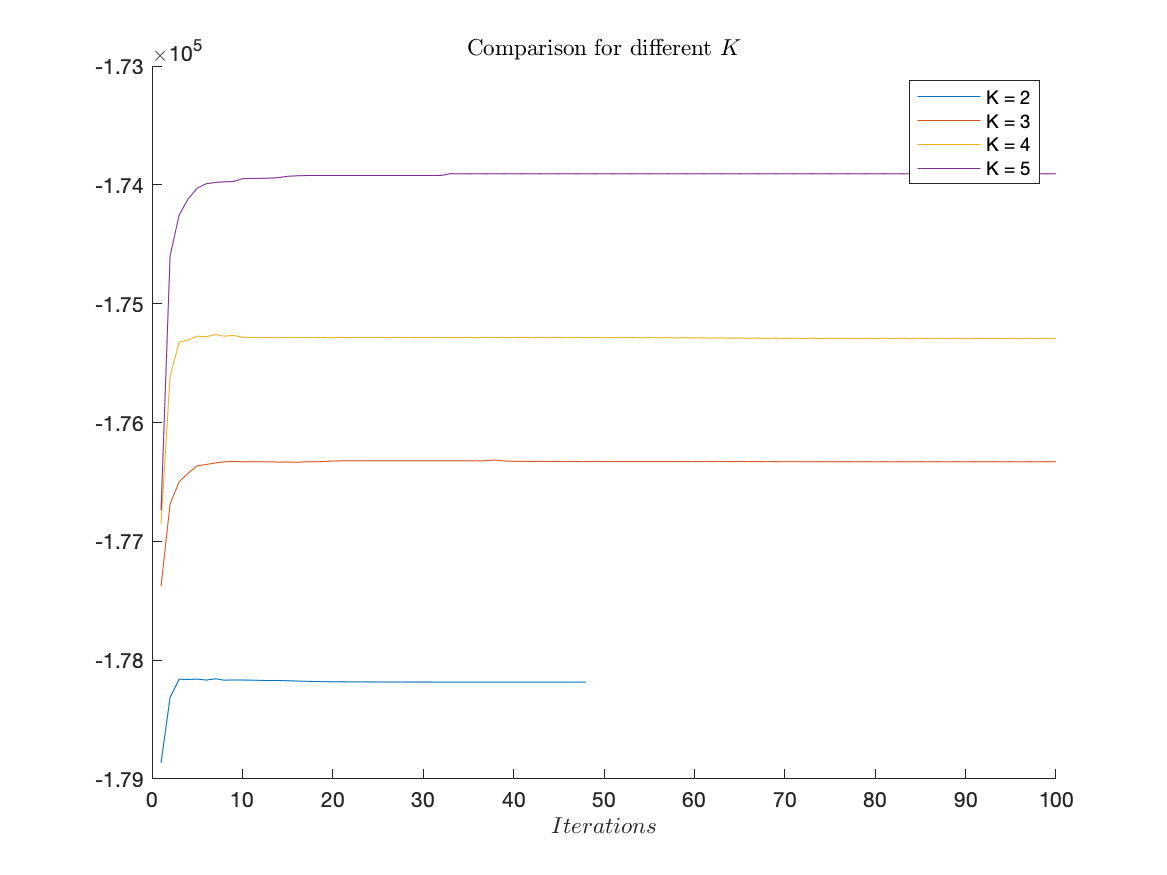
\includegraphics[width=0.8\textwidth]{images/ll_comparison.png}
	\caption{Comparison of the log-likelihoods for K $\in$ [2,5]}
	\label{fig:ll_comparison}
\end{figure}

Next, Figure \ref{fig:Q_all} displays like Figure \ref{fig:ll_comparison} all log-likelihood curves but in this case separated. \\

\begin{figure}[h]
	\centering
	\begin{subfigure}{0.45\textwidth}
		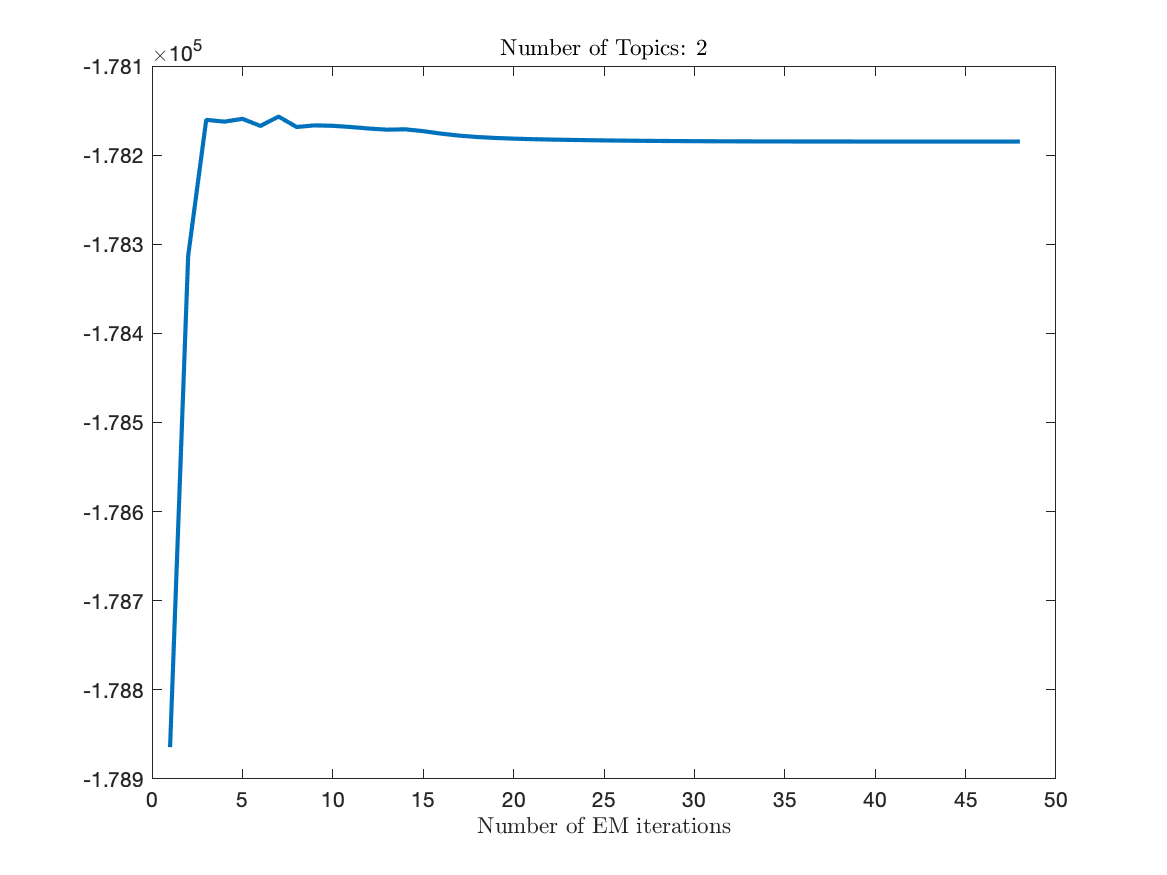
\includegraphics[width=\textwidth]{images/Q_2_topics.png}
		\caption{Log-likelihood curve for K = 2}
		\label{fig:Q2}
	\end{subfigure}
	~	
	\begin{subfigure}{0.45\textwidth}
		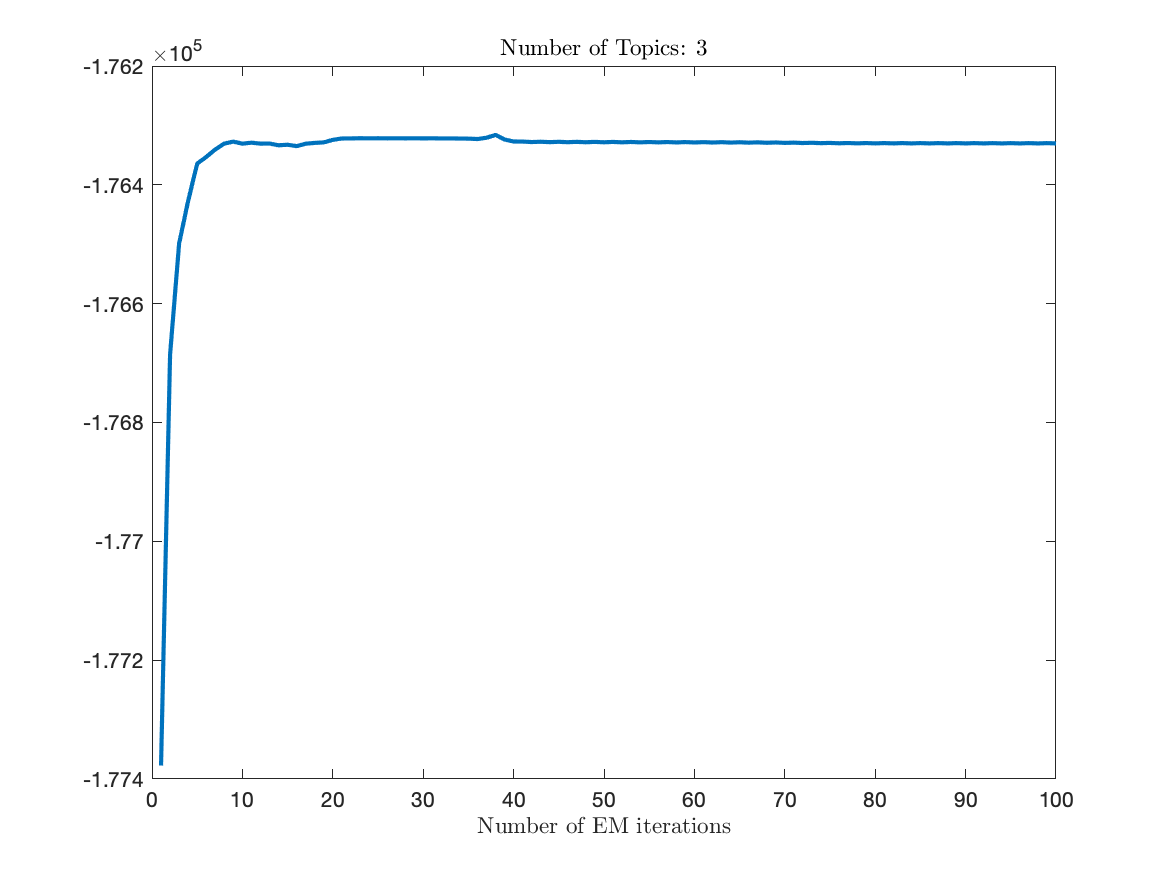
\includegraphics[width=\textwidth]{images/Q_3_topics.png}
		\caption{Log-likelihood curve for K = 3}
		\label{fig:Q3}
	\end{subfigure}
		~	
	\begin{subfigure}{0.45\textwidth}
		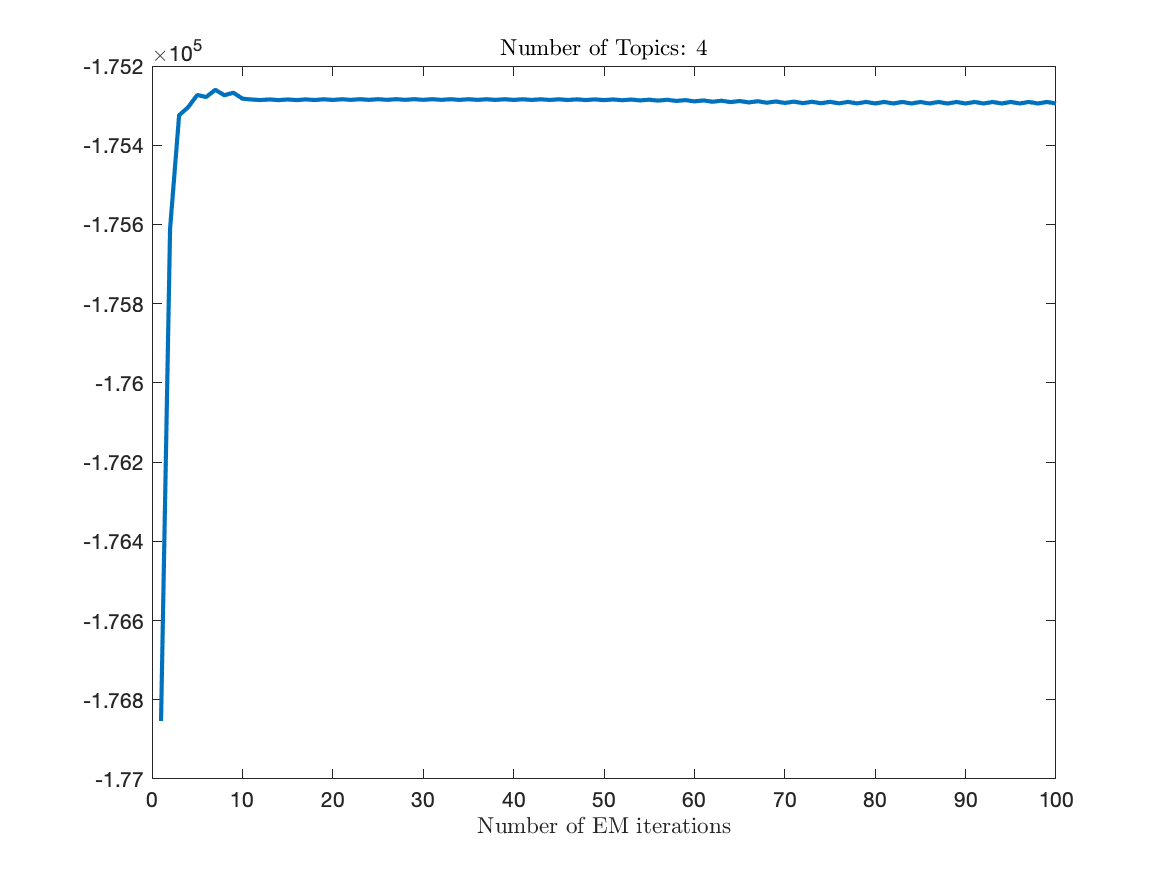
\includegraphics[width=\textwidth]{images/Q_4_topics.png}
		\caption{Log-likelihood curve for K = 4}
		\label{fig:Q4}
	\end{subfigure}
		~	
	\begin{subfigure}{0.45\textwidth}
		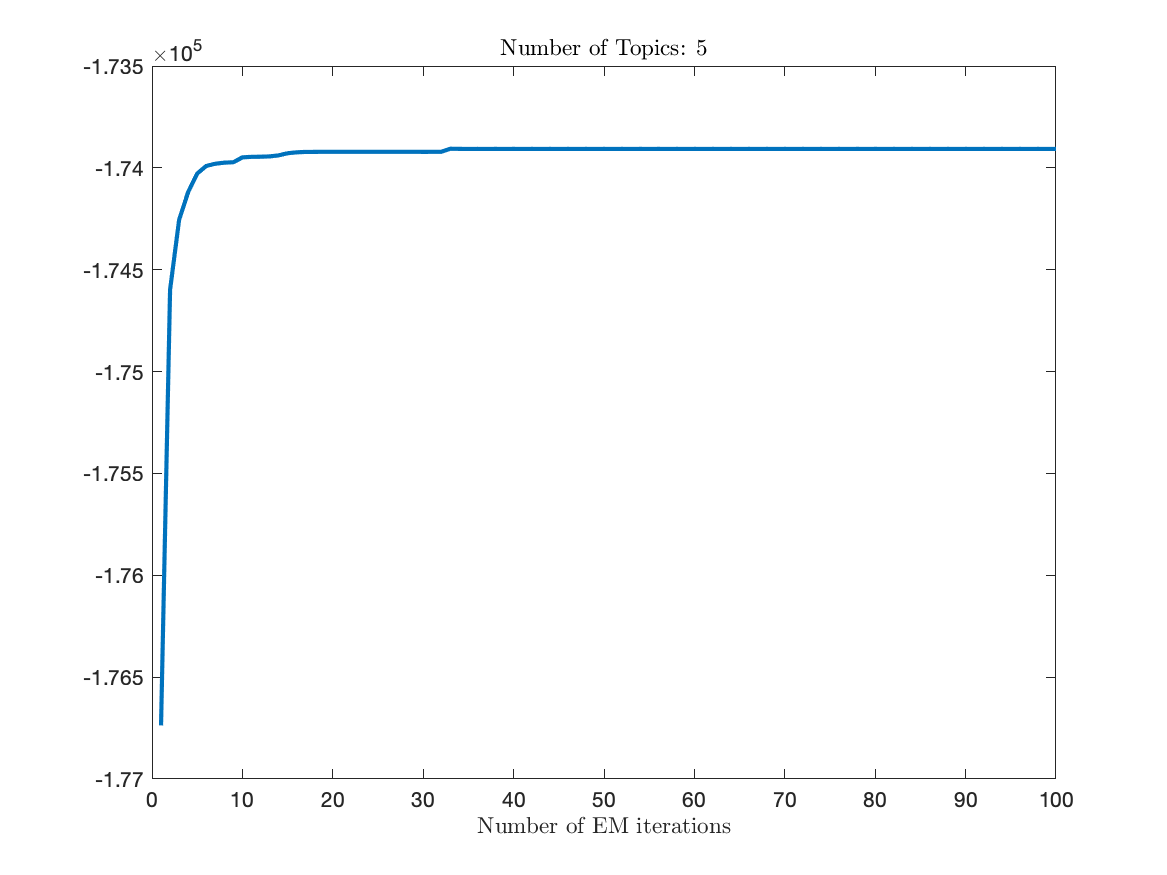
\includegraphics[width=\textwidth]{images/Q_5_topics.png}
		\caption{Log-likelihood curve for K = 5}
		\label{fig:Q5}
	\end{subfigure}
	\caption{Separated log-likelihood curves for K $\in$ [2,5]}
	\label{fig:Q_all}
\end{figure}

\noindent This last set of figures, which include from Figure \ref{fig:viterbi_2} until Figure \ref{fig:viterbi_5}, show the estimated states for sequences for K $\in$ [2,5].

\begin{figure}[h]
	\centering
	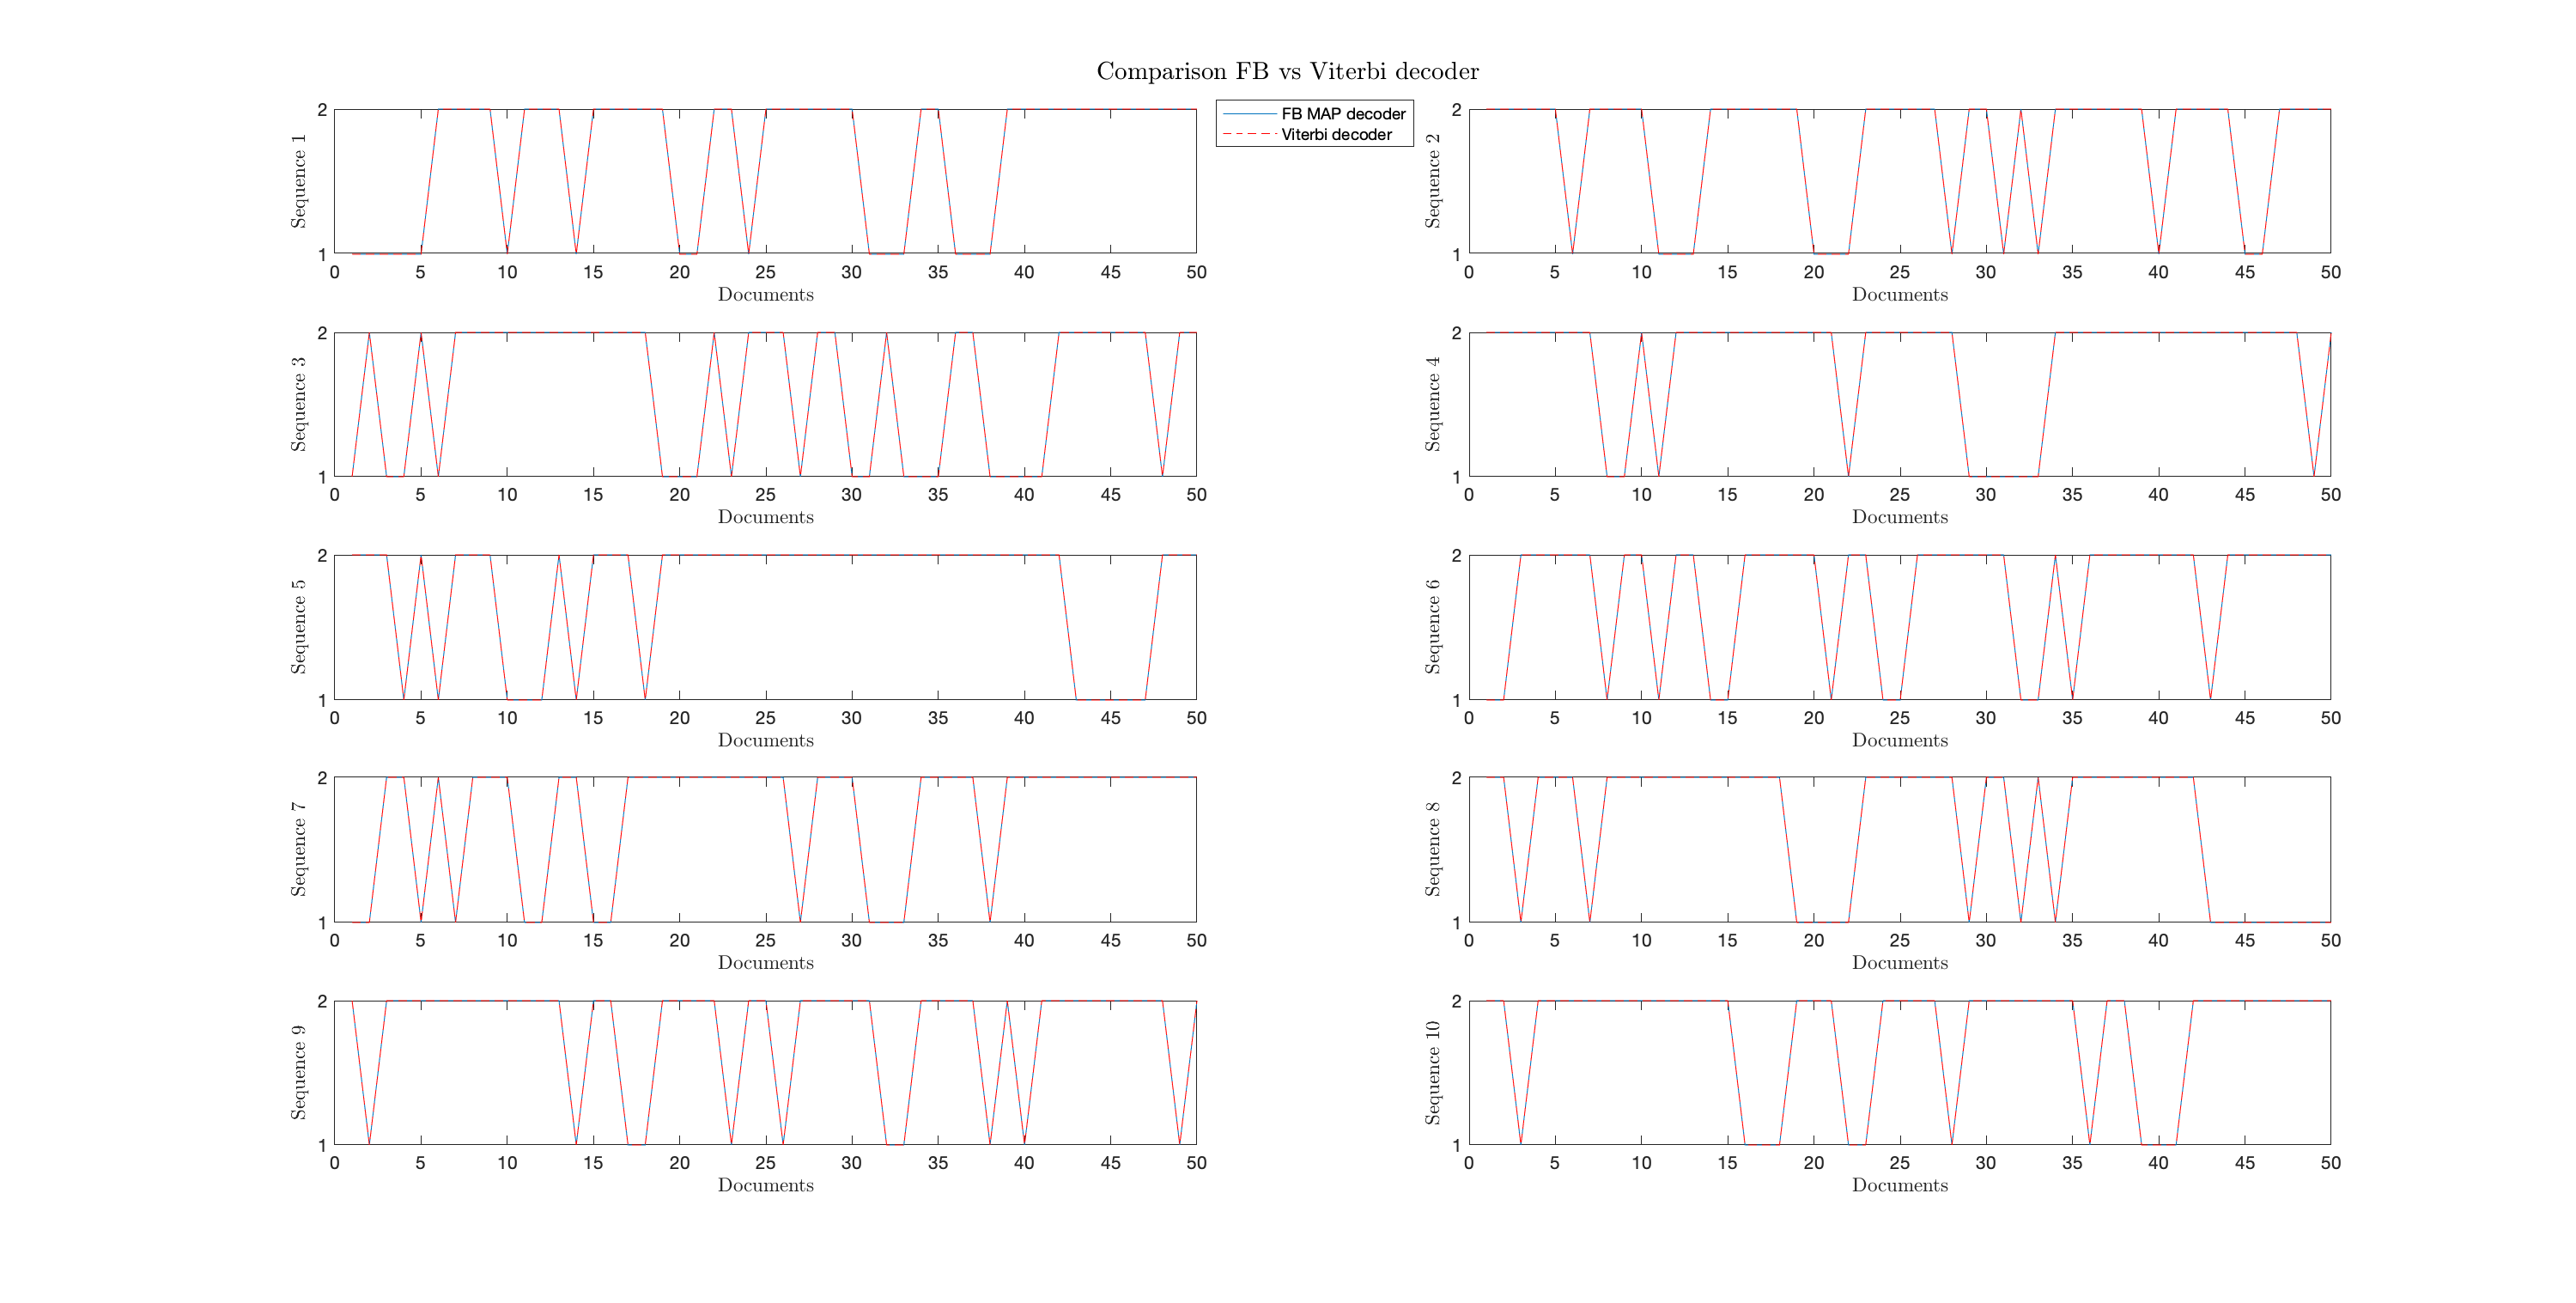
\includegraphics[width=\textwidth]{images/comparison_FB_Viterbi_K_2.png}
	\caption{Forward Backward (MAP) and Viterbi (ML) estimations for K = 2}
	\label{fig:viterbi_2}
\end{figure}

\begin{figure}[h]
	\centering
	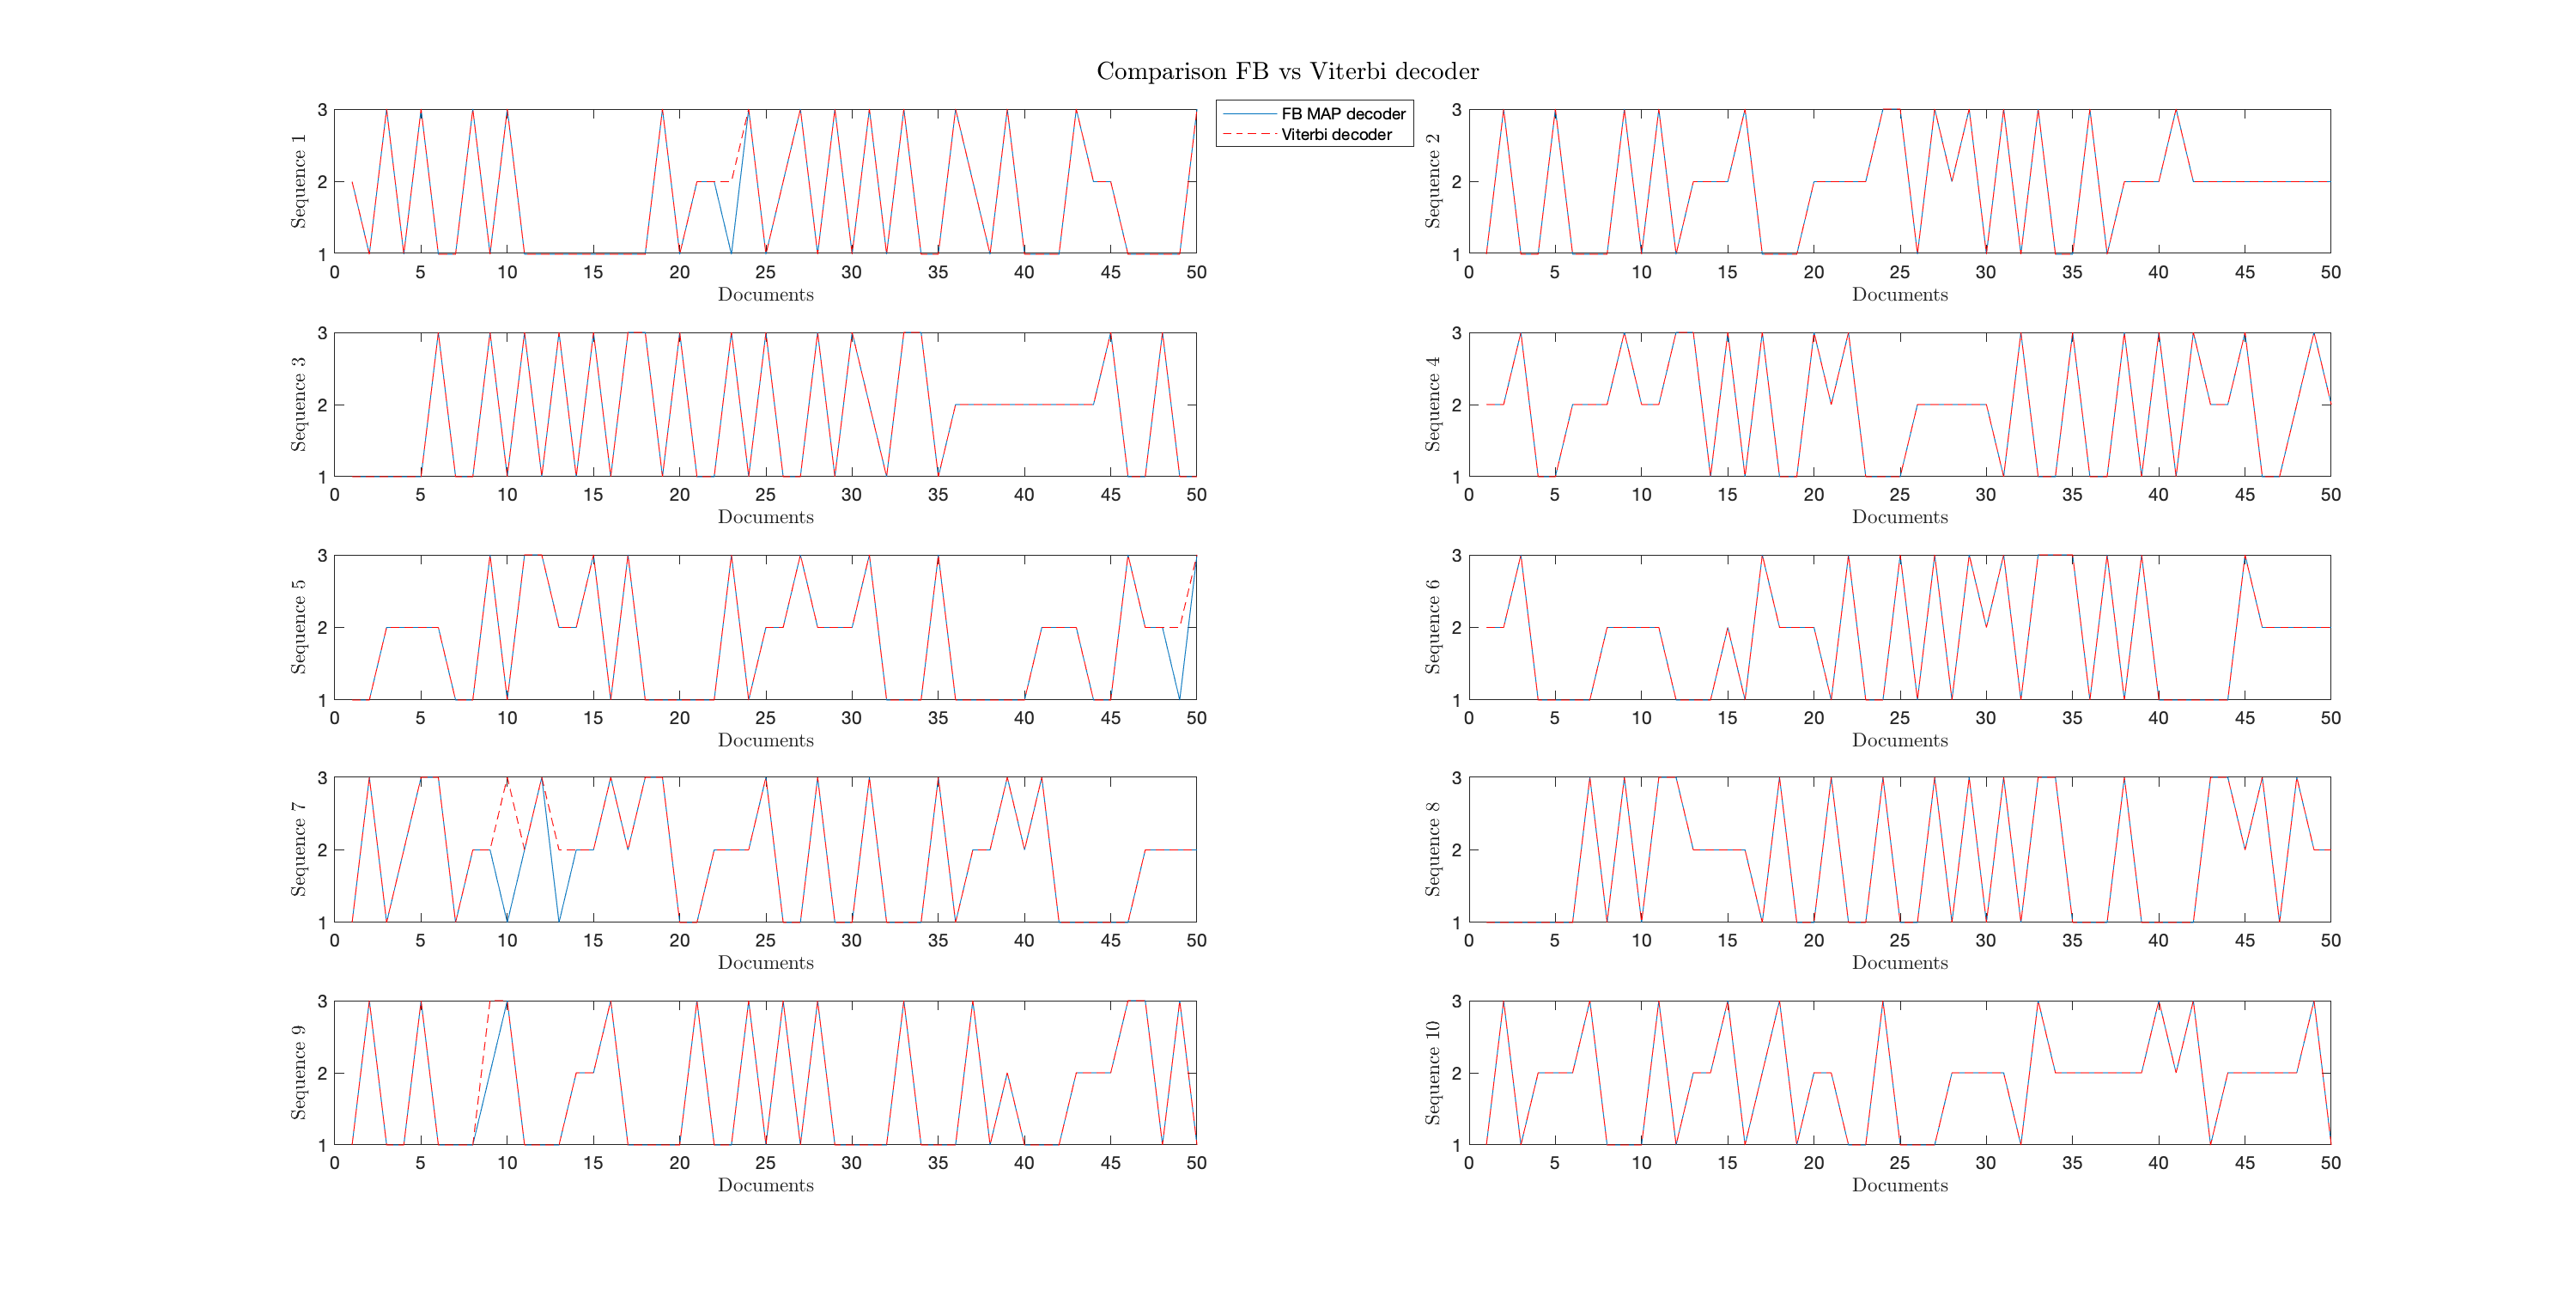
\includegraphics[width=\textwidth]{images/comparison_FB_Viterbi_K_3.png}
\caption{Forward Backward (MAP) and Viterbi (ML) estimations for K = 3}
	\label{fig:viterbi_3}
\end{figure}

\begin{figure}[h]
	\centering
	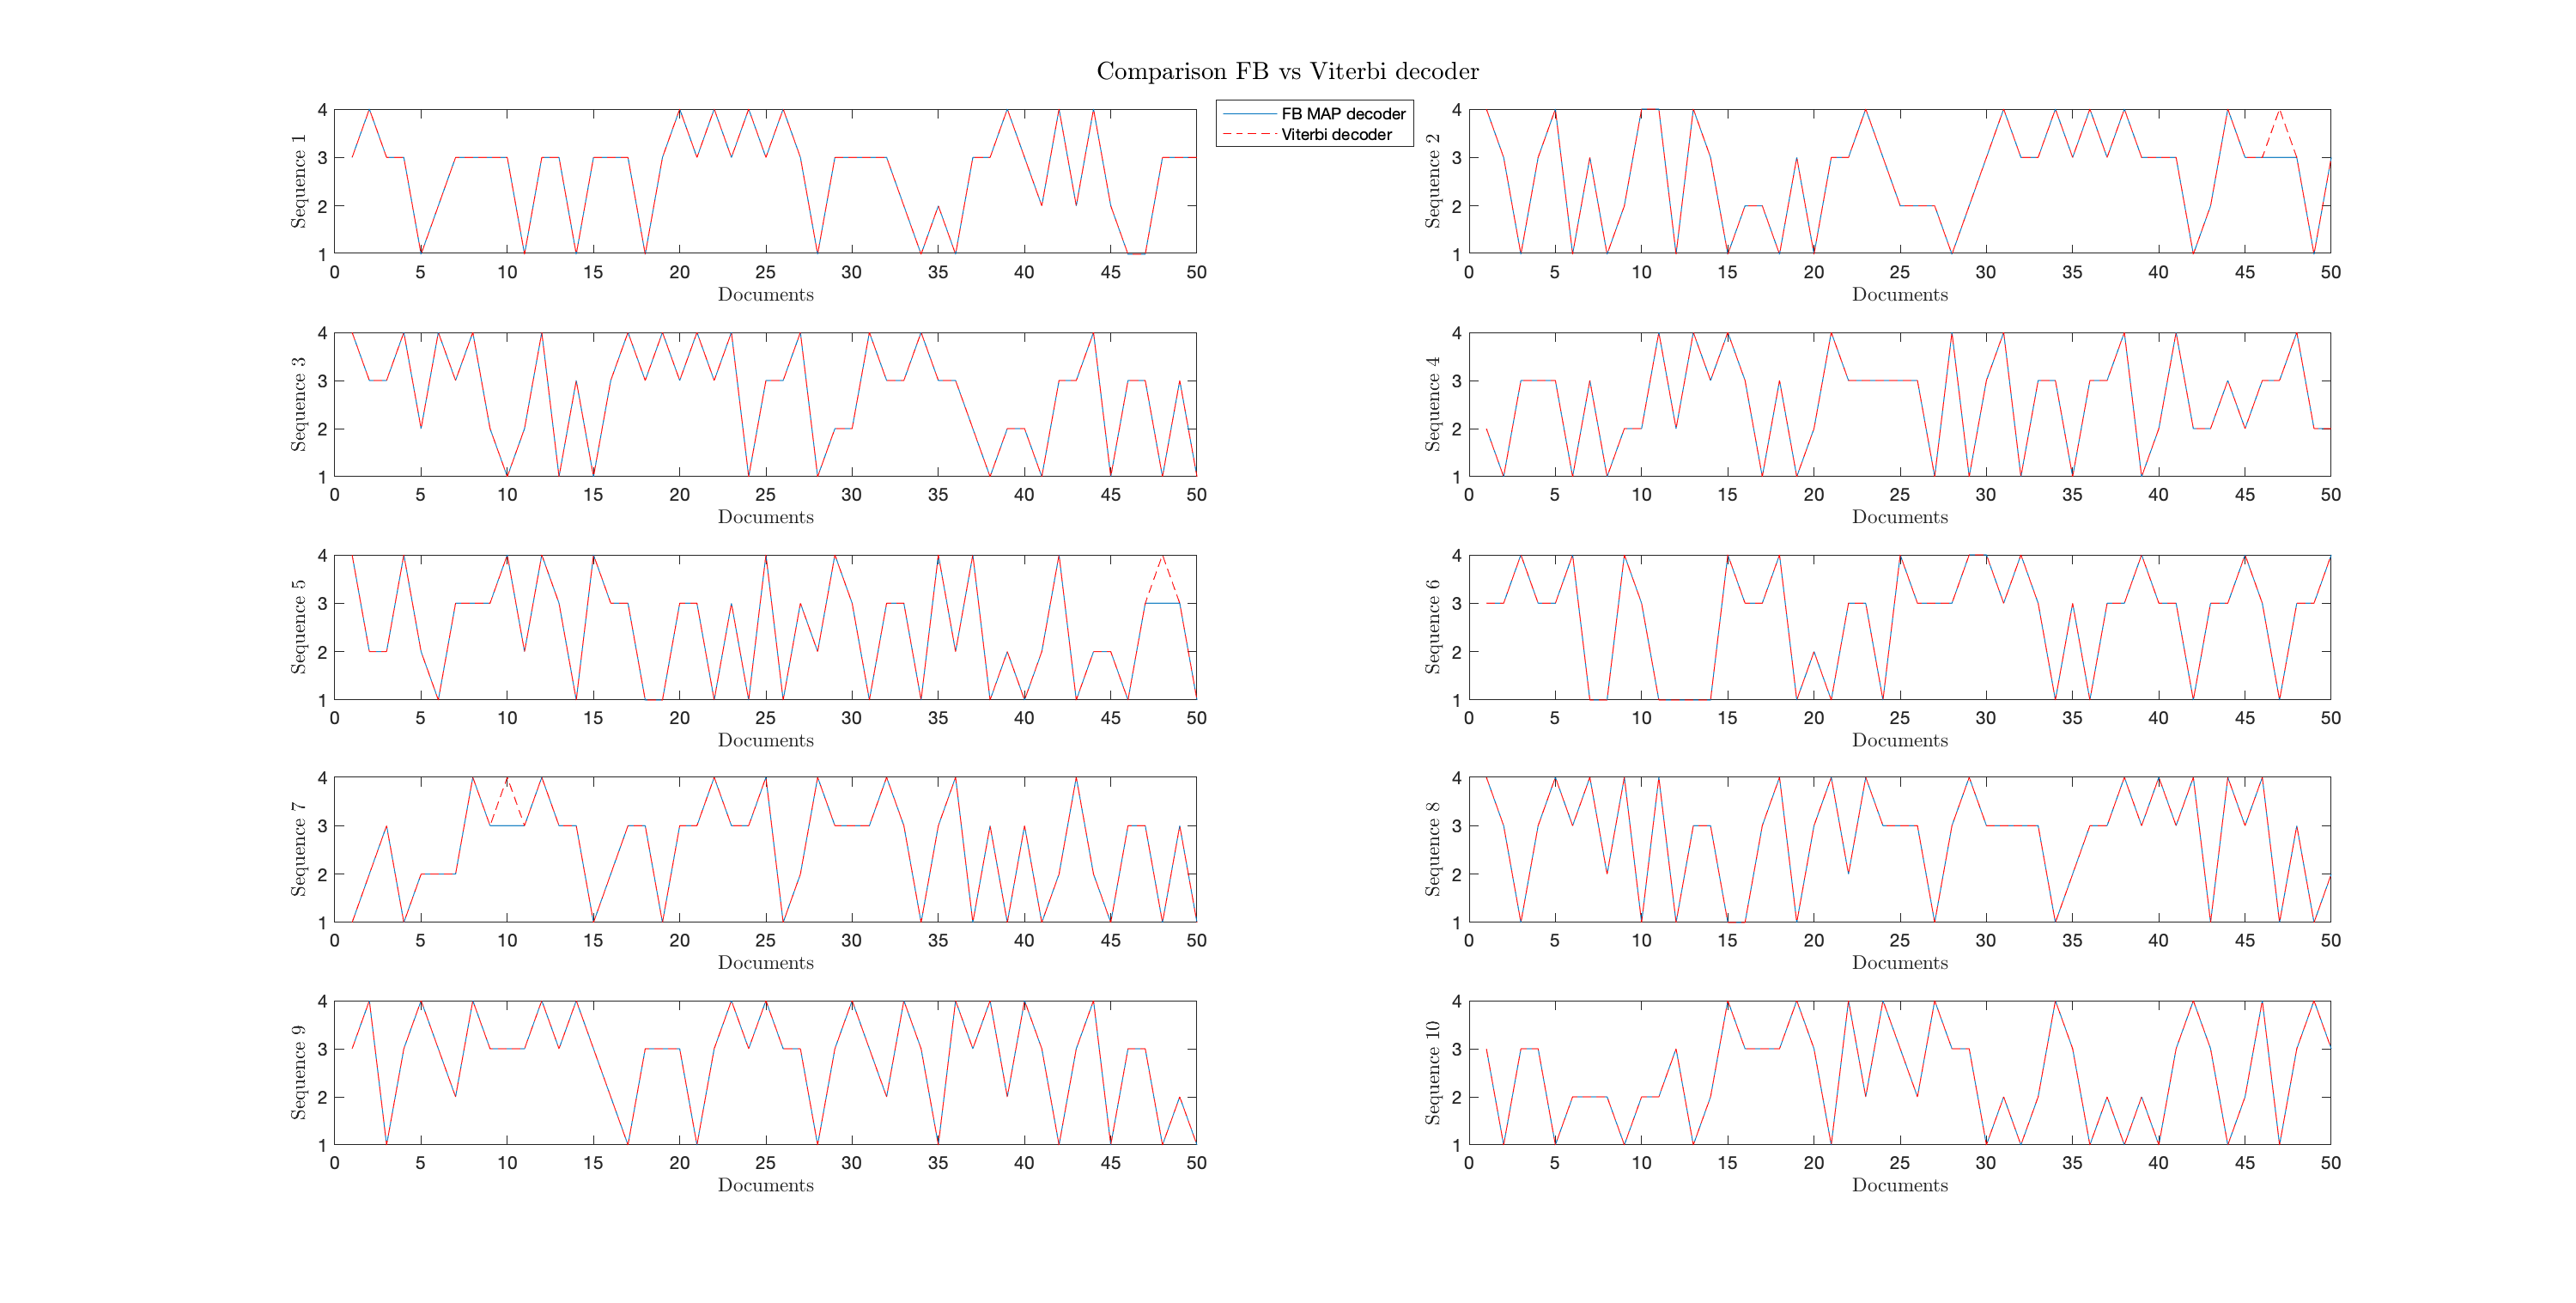
\includegraphics[width=\textwidth]{images/comparison_FB_Viterbi_K_4.png}
	\caption{Forward Backward (MAP) and Viterbi (ML) estimations for K = 4}
	\label{fig:viterbi_4}
\end{figure}

\begin{figure}[h]
	\centering
	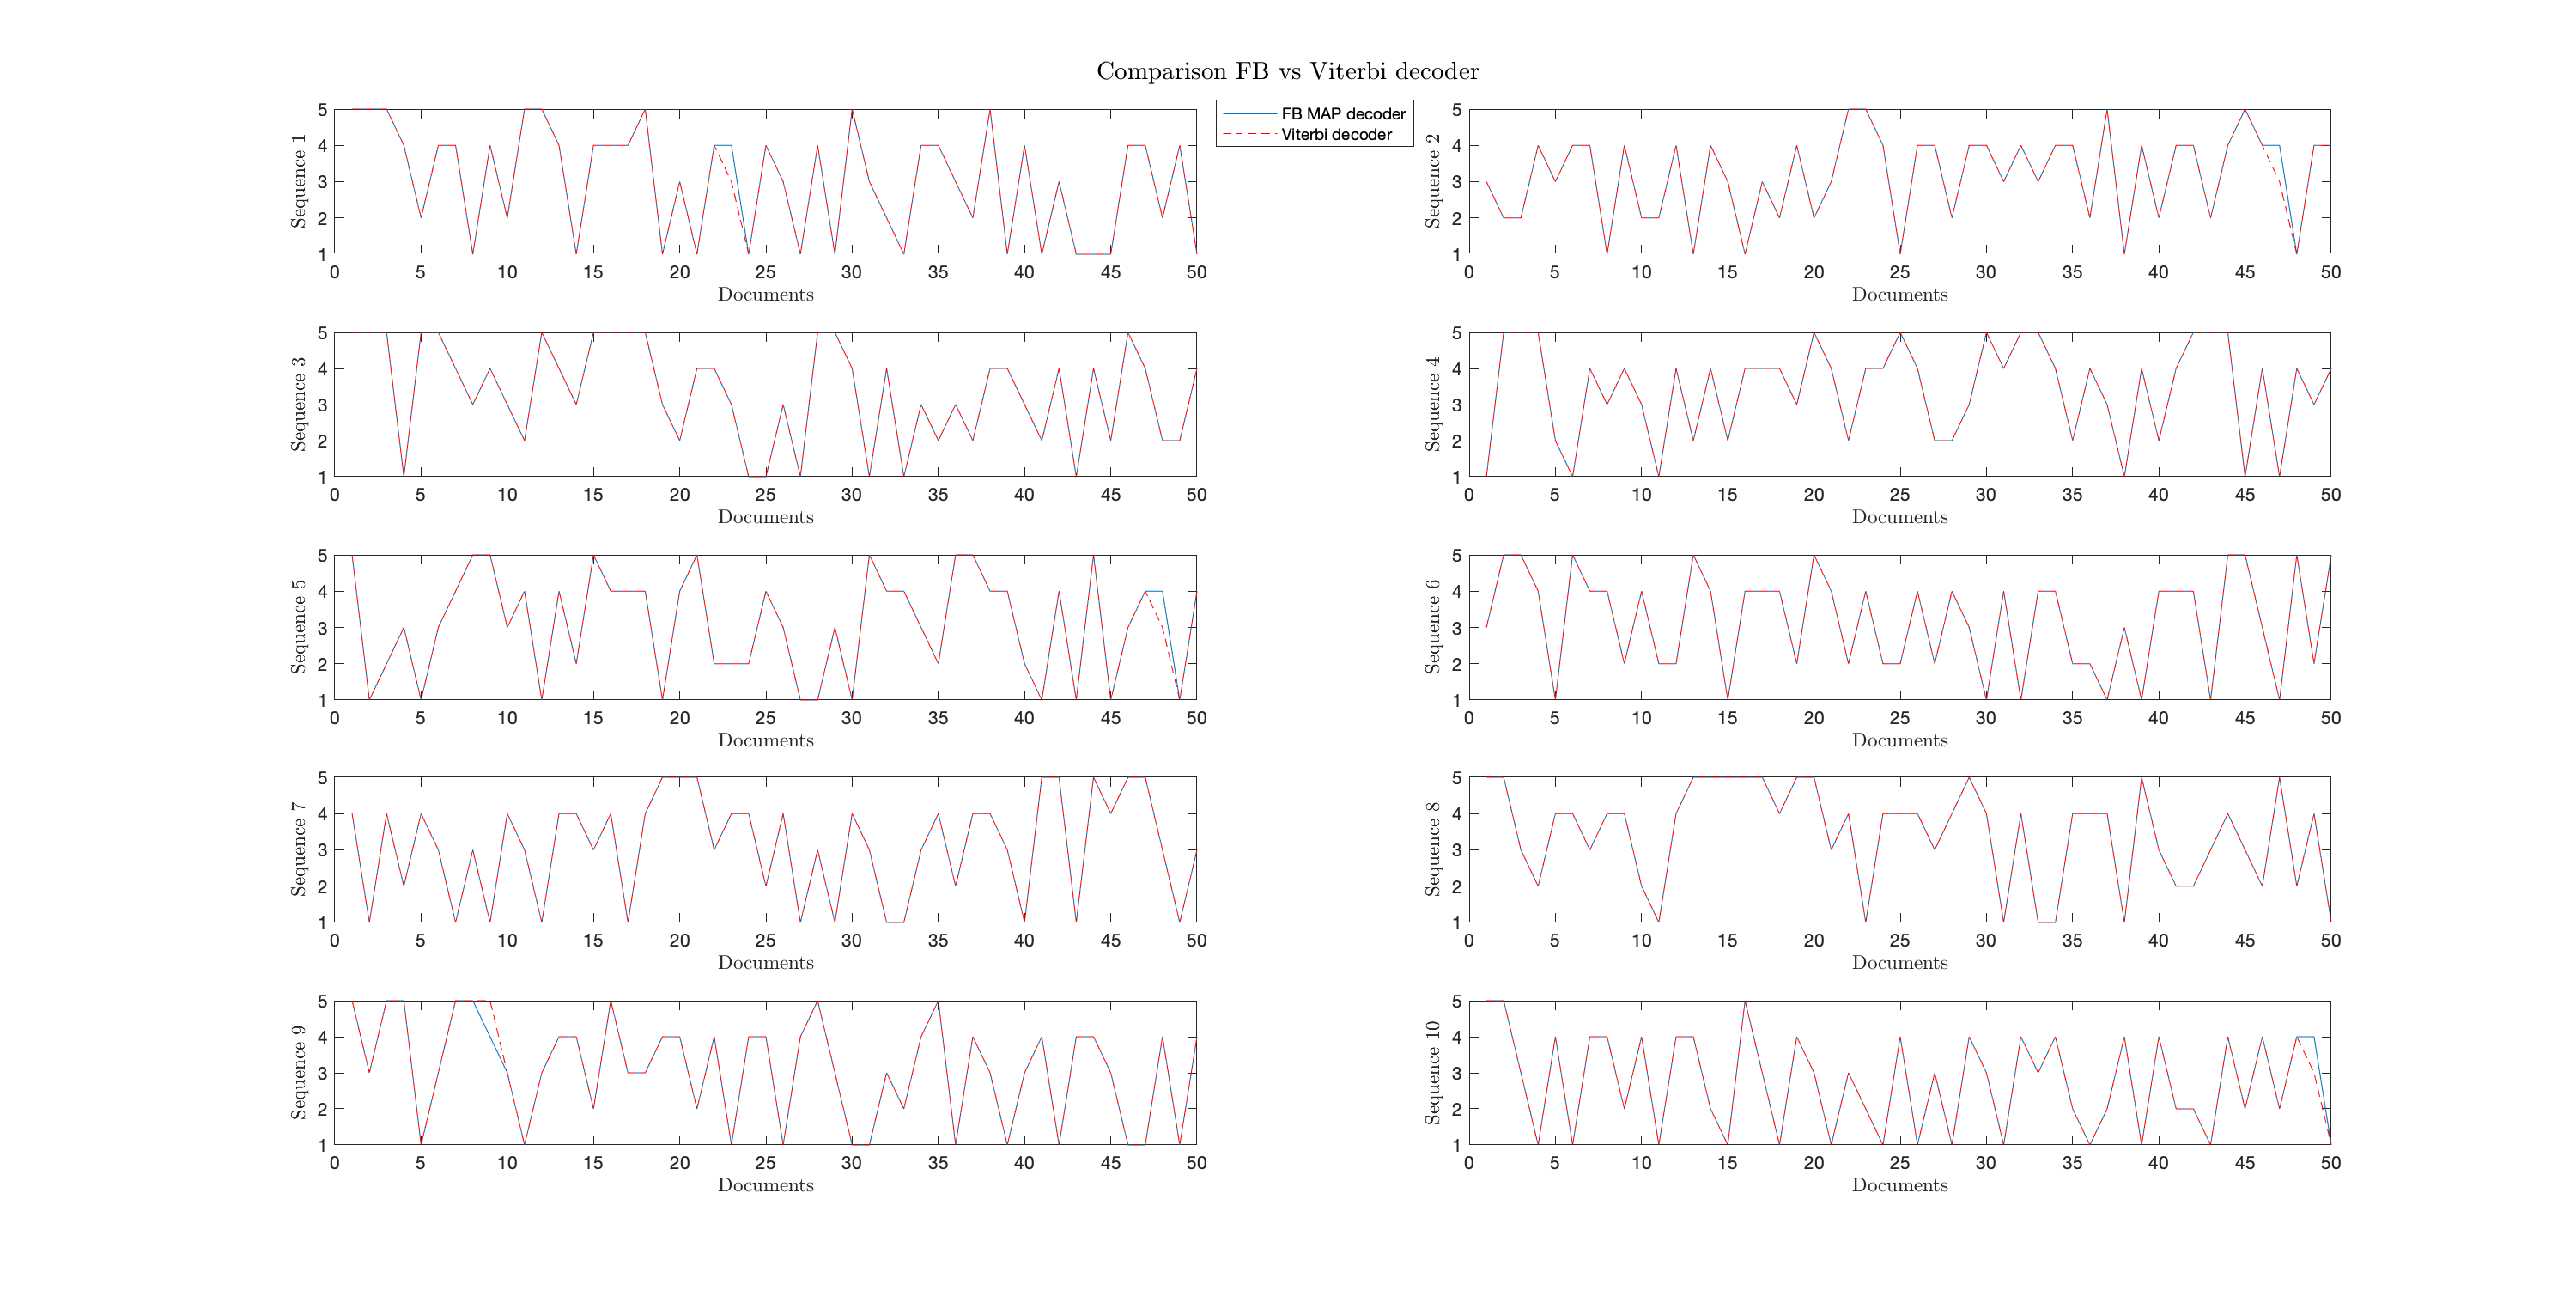
\includegraphics[width=\textwidth]{images/comparison_FB_Viterbi_K_5.png}
	\caption{Forward Backward (MAP) and Viterbi (ML) estimations for K = 5}
	\label{fig:viterbi_5}
\end{figure}

\section{Final Thoughts}
By looking at the plots, we can see a proper behaviour of of the curves (which begin growing up and later they stabilize around some fixed value) and the algorithms. Both experiments seem to have a similar performance, they show that they reach almost always the same states for all the sequences. And at last, a bigger number of K increases the complexity of the model, which includes the number of states among other things, but gives a better performance with a bigger log-likelihood curve.
\end{document}
